\documentclass{article}
\usepackage[utf8]{inputenc}

\title{AAA Project}
%\author{Liron Mizrahi - 708810, Daniel da Silva - 738215, Jan Badenhorst - 707831}
\date{September 2016}

\author{
  Liron Mizrahi\\
  \texttt{708810}
  \and
  Daniel da Silva\\
  \texttt{738215}
  \and
  Jan Badenhorst\\
  \texttt{707831}
}


\usepackage{natbib}
\usepackage{graphicx}
\usepackage{algorithmic}
\usepackage{float}
\usepackage{hyperref}

\begin{document}

\maketitle

\section{Aims}
The problem proposed is to solve Sudoku's using the Backtracking Algorithm and to verify the theoretical analysis of the algorithm using empirical analysis.

\section{Summary of Theory}
A Backtracking algorithm is a type of brute force algorithm that incrementally builds candidates to the solution. If a candidate is found to be invalid, the algorithm 'backtracks' and deletes it. This only happens if the algorithm determines that the candidate cannot possibly lead to a solution.

\section{Experimental Methodology}
\subsection{Understanding the theoretical analysis}
The time complexity for this algorithm can be seen by working backwards from a single blank square. If there is only one blank square, then in the worst case there are $n$ possibilities that must be worked through. If there are two blank squares, then there are $n$ possibilities for the first square and $n$ possibilities for the second square corresponding to each of the possibilities for the first square. If there are three blank squares, then there are $n$ possibilities for the first blank. Each of those possibilities will lead to a puzzle with two blank squares that have $n^2$ possibilities.
The algorithm performs a depth first search through all the possible solutions. So carrying on in this way, the worst case complexity will end up being $O(n^m)$, where $n$ is the number of possibilities for each square and $m$ is the number of blank squares.
The best case for this algorithm would be where all the missing blocks are low values. If that happens to be the case then there will be significantly less backtracking than if the missing values were higher. Therefore the worst case would be where the missing values are all higher values. The growth of both best and worst case would still be exponential except with lower and higher constants involved.

\newpage

\subsection{Deciding on Appropriate Hardware and Programming Language}
We are more interested in the rate of growth of the performance of the algorithm than the actual running times and as such the specific hardware used will not be a relevant factor so long as the tests are run on the same hardware. However, the programming language that has been chosen is C++, as it is much easier and more reliable to time the algorithm with the OpenMP library, rather than Java's timing implementations. Also, Java would be easier to use for this sort of problem but the Garbage Collector may change results drastically and lead to incorrect results.

\subsection{Deciding on Appropriate Data Structures}
The data structure used is a three dimensional array. This is to store multiple sudokus (6 from the number of sudokus per text file). Prior to being passed to the backtracking algorithm, however, a sudoku is copied into a new two dimensional array. This is to reduce the memory access times required to reference the three dimensional array.

\newpage

\subsection{Implement the Algorithm}

    \begin{algorithmic}[1]
    %\Function{Increment}{$a$}
    
    \STATE Solve($int matrix[][]$)
        \STATE int $row$
        \STATE int $column$
\newline
        \IF {there are no empty squares} 
            \RETURN $true$
        \ENDIF
\newline
        \FOR{$value$ from $0$ \TO $9$}
            \IF{there are no numbers in same row, column and 3x3 square as $value$}
                \STATE $matrix[row][column]\gets value$
            
                \IF{Solve($matrix$)}
                    \RETURN $true$
                \ENDIF
                
                \STATE $matrix[row][column]\gets 0$
            \ENDIF
        \ENDFOR
\newline
        \RETURN $false$
    \STATE EndSolve
    %\EndFunction
\newline
    \end{algorithmic}

The algorithm above takes in a sudoku as a 2D matrix. The if statement on line 4 checks if there are any empty blocks in the matrix, if there are then $row$ and $column$ are assigned to the corresponding block. If there are no empty blocks then the sudoku is complete. 

The for loop on line 10 will iterate through the values $1$ to $9$ for the corresponding empty block. The if statement underneath checks if the current value can be placed in the block without breaking any of the rules of the sudoku. If it can be placed there then $matrix[row][column]$ is updated to the value.

The if statement on line 10 will recursively call the Solve function for $matrix$ with the newly inserted variable.
If the any function call reaches line 13 then it means the current setup has failed and that the latest value must be backtracked. This line will reset the current block to 0. Line 16 is the line that invokes backtracking. When a $false$ value is returned then the previous block that was updated must be tried again for the other values it has not tried yet. If every function call returns true then the sudoku has been solved. If the first function call returns false then the sudoku has no solution.

\newpage

\subsection{Create the Data}
Data was generated using the website https://kjell.haxx.se/sudoku/. A field of 6 sudokus was generated for each number of given numbers from 17 up to 35. Another website (https://regex101.com/) was then used to convert the sudokus into the required format.

A metric was designed to approximate the difficulty of the puzzles using the formula: \[\frac{number\_empty\_cells}{max\_number\_completed\_cells\_(block/row/column)}\]

This metric is useful in approximating the difficulty of the puzzle and was found to agree with the difficulty levels quoted by the website for each puzzle. However, our main analysis uses the number of empty cells vs time. This metric is just an attempt at evaluating what makes a sudoku difficult.

\newpage

\section{Presentation of Results}
\subsection{Number of empty cells}
Firstly we examine the graphs of time vs number of empty cells.

\begin{figure}[H]
	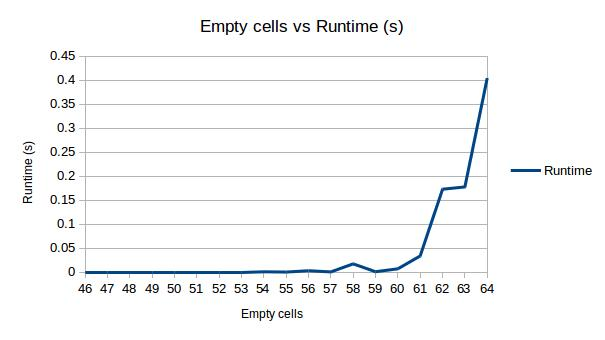
\includegraphics[width=0.9\linewidth, height=5cm]{graphs_outputs/EmptycellsVSTimeAggregated.jpg}
	\caption{Aggregated data Empty cells vs time}
\end{figure}


\begin{figure}[H]
	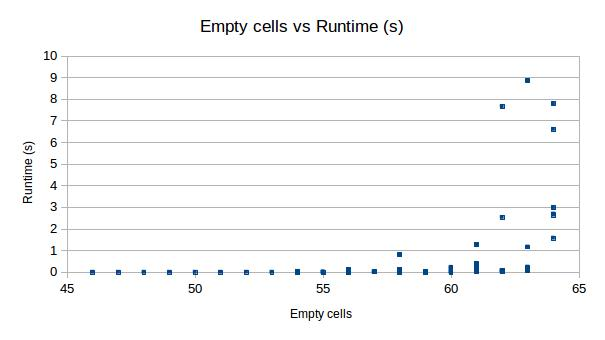
\includegraphics[width=0.9\linewidth, height=5cm]{graphs_outputs/EmptycellsVSTimeScatter.jpg}
	\caption{Scatter plot data Empty cells vs time}
\end{figure}

\newpage

\subsection{Difficulty metric}
We now examine the test metric graphs to evaluate how good of an approximation it is for difficulty.

\begin{figure}[H]
	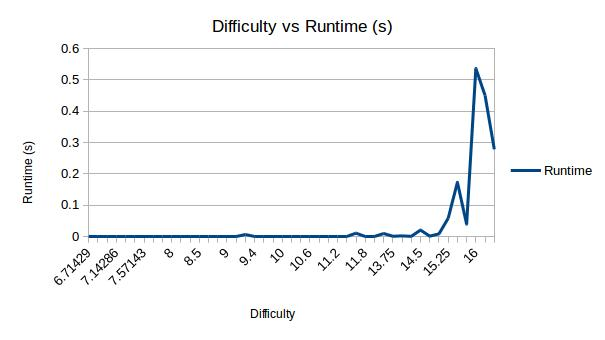
\includegraphics[width=0.9\linewidth, height=5cm]{graphs_outputs/DifficultyVSTimeAggregated.jpg}
	\caption{Aggregated data Difficulty vs time}
\end{figure}


\begin{figure}[H]
	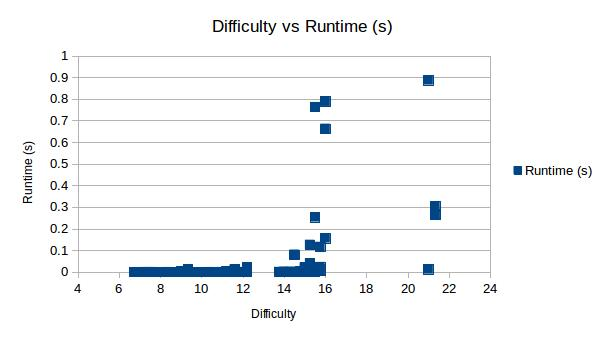
\includegraphics[width=0.9\linewidth, height=5cm]{graphs_outputs/DifficultyVSTimeScatter.jpg}
	\caption{Scatter plot data Difficulty vs time}
\end{figure}

\newpage

\section{Interpretation of Results}
\subsection{Number of empty cells}
It is clear from figure 1 that there is a sharp increase in runtime from 61 empty cells to 64 empty cells. This growth is exponential and would likely continue for sudokus with a higher number of empty cells. A somewhat small increase in runtime can be seen from 62 to 63 empty cells. We can ascertain that this is variation due to a few outliers as seen in figure 2. The number of sudokus taken into consideration for a given number of cells is only 6, so variations like these are to be expected. There is another variation in figure 1 at 58 empty cells. We can again ascertain that this is due to, in this case, a single outlier as seen in figure 2. There is a lot of variation in this problem as for some sudokus the algorithm may be 'lucky' and guess right multiple times without having to actually backtrack. Given that there are only 6 sudokus per number of empty cells, the relationship is considerably strong. It is also important to note the small runtimes for 46 to 57 empty cells, which provide small changes that cannot be viewed in figure 1 due to the scaling. Refer to figure 5 below for the graph of that region.

\begin{figure}[H]
	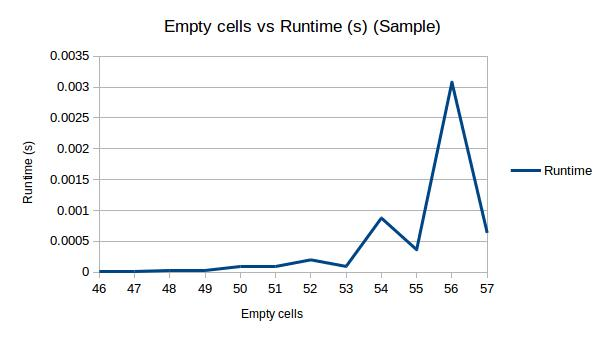
\includegraphics[width=0.9\linewidth, height=5cm]{graphs_outputs/EmptycellsVSTimeAggregated(Sample).jpg}
	\caption{Aggregated data Empty cells vs time for 46-57}
\end{figure}

Here we see an exponential relation as well, which again, appears as a straight line on the graph in figure 1. This really outlines the magnitude with which the runtime increased in figure 1.

\newpage

\subsection{Difficulty metric}
The difficulty metric mostly mirrors the number of empty cells graphs, however there are much larger variations in the graphs. The metric takes into account difficulty a human would have in solving a sudoku as opposed to what the algorithm might struggle with. It does not seem to provide a better approximation than the number of empty cells. Notice the large variation right at the end of the graph (at around 21 difficulty units), this is clearly a sudoku being rated as quite difficult when it should not be considered as such. This is why the metric is not considered in the empirical analysis.

\section{Relate results to Theory}
As seen in figure 5, there is a clear exponential growth as the number of empty cells grows. Also by figure 3, it is clear that there is an exponential growth as the difficulty of the sudoku increases. As stated above the time complexity of $O(n^m)$ agrees with the graphs obtained.

\section{Conclusion}
As shown by the graphs and the theoretical analysis, the time complexity of the backtracking algorithm is $O(n^m)$, which is exponential. This is not a very efficient algorithm, but when working with 9x9 grids the complexity is not very obvious. The backtracking approach to Sudoku puzzles should perform a lot more efficiently than primitive brute force as it eliminates a lot of possible attempts.

\section{Acknowledgments}
Thank you to Kjell Ericson for the test data which is created on demand at https://kjell.haxx.se/sudoku/.

\section{References}
\url{https://en.wikipedia.org/wiki/Sudoku_solving_algorithms} \\
\url{https://codemyroad.wordpress.com/2014/05/01/solving-sudoku-by-backtracking/}

\end{document}
